\documentclass{article}
\usepackage[utf8]{inputenc}
\usepackage[vietnamese,english]{babel}
\usepackage{times}
\usepackage{amsmath,amssymb}
\usepackage{tabularx}
\usepackage{graphicx}
\usepackage{xcolor}
\usepackage{tikz}
\usetikzlibrary{shapes.geometric, arrows.meta, positioning, calc, backgrounds}

\usepackage[
  paperwidth=29.7cm,
  paperheight=16.706cm,
  top=0.8cm,
  bottom=0.8cm,
  left=1.0cm,
  right=1.0cm,
  footskip=0pt,
  headheight=0pt,
  headsep=0pt
]{geometry}

\pagestyle{empty}
\setlength{\parindent}{0pt}
\setlength{\parskip}{0pt}

% Color definitions
\definecolor{brandGreen}{RGB}{16, 149, 114}
\definecolor{lightGreen}{RGB}{236, 253, 245}
\definecolor{borderGreen}{RGB}{110, 231, 183}
\definecolor{darkGreen}{RGB}{6, 95, 70}

\definecolor{brandBlue}{RGB}{30, 64, 175}
\definecolor{lightBlue}{RGB}{239, 246, 255}
\definecolor{borderBlue}{RGB}{147, 197, 253}
\definecolor{darkBlue}{RGB}{30, 58, 138}

\definecolor{alertBg}{RGB}{254, 243, 199}
\definecolor{alertBorder}{RGB}{245, 158, 11}
\definecolor{alertText}{RGB}{146, 64, 14}

\definecolor{badgeBg}{RGB}{241, 245, 249}
\definecolor{badgeBorder}{RGB}{203, 213, 225}

\begin{document}
\selectlanguage{vietnamese}

\begin{tikzpicture}[remember picture, overlay]
  % Full slide background
  \fill[color=white] (current page.south west) rectangle (current page.north east);
  
  % Top accent line
  \fill[color=brandBlue] (current page.north west) rectangle ($(current page.north east) + (0,-0.25cm)$);
\end{tikzpicture}

% ---------------- HEADER ----------------
\vspace*{-0.2cm}
\begin{center}
  \tikz[baseline]{
    \node[fill=lightGreen, draw=brandGreen, rounded corners=3pt, inner sep=5pt] {
      {\fontsize{11}{13}\selectfont \textbf{\color{darkGreen}$\star$ KHOA HỌC TỰ NHIÊN • SINH HỌC $\star$}}
    };
  }\\[0.25cm]
  {\fontsize{22}{26}\selectfont \textbf{VÌ SAO CƠ THỂ ĐA BÀO CẦN NHIỀU TẾ BÀO CHUYÊN HOÁ?}}\\[0.2cm]
  {\fontsize{12}{15}\selectfont \textit{\color{gray!80!black}So sánh đặc điểm trao đổi chất \& quy luật tỉ lệ diện tích bề mặt/thể tích ($S/V$) giữa cơ thể đơn bào và cơ thể đa bào}}
\end{center}

\vspace{0.35cm}

% ---------------- 2 COMPARISON COLUMNS ----------------
\begin{tabularx}{\textwidth}{@{} X @{\hspace{0.7cm}} X @{}}

% ===== COLUMN 1: CƠ THỂ ĐƠN BÀO =====
\begin{tikzpicture}
  \node[draw=borderGreen, fill=lightGreen!30, rounded corners=8pt, line width=1.2pt, inner sep=0pt] (card1) {
    \begin{minipage}{13.4cm}
      % Card Title
      \begin{tikzpicture}
        \node[fill=brandGreen, text=white, minimum width=13.4cm, minimum height=1.1cm, rounded corners=7pt] {
          {\fontsize{14}{17}\selectfont \textbf{CƠ THỂ ĐƠN BÀO (Ví dụ: Trùng biến hình)}}
        };
      \end{tikzpicture}
      
      \vspace{0.25cm}
      
      \begin{minipage}[t]{8.4cm}
        \fontsize{10.5}{15}\selectfont
        \begin{itemize}
          \setlength{\itemsep}{7pt}
          \setlength{\leftmargin}{0.3cm}
          \item[\color{brandGreen}$\blacktriangleright$] \textbf{\color{darkGreen}Kích thước cơ thể:} Rất nhỏ (kích thước hiển vi).
          \item[\color{brandGreen}$\blacktriangleright$] \textbf{\color{darkGreen}Tỉ lệ $S/V$ (Diện tích / Thể tích):} \textbf{\color{red!70!black}RẤT LỚN} (diện tích bề mặt tiếp xúc môi trường lớn so với thể tích).
          \item[\color{brandGreen}$\blacktriangleright$] \textbf{\color{darkGreen}Cơ chế trao đổi chất:} Các chất dinh dưỡng và chất thải \textbf{dễ dàng khuếch tán trực tiếp qua màng sinh chất}.
          \item[\color{brandGreen}$\blacktriangleright$] \textbf{\color{darkGreen}Tốc độ trao đổi chất:} Nhanh chóng, đáp ứng đủ và kịp thời mọi nhu cầu sống của tế bào.
          \item[\color{brandGreen}$\blacktriangleright$] \textbf{\color{darkGreen}Mức độ chuyên hoá:} \textbf{KHÔNG CÓ tế bào chuyên hoá} (toàn bộ hoạt động sống do 1 tế bào duy nhất đảm nhận).
        \end{itemize}
      \end{minipage}%
      \hfill
      \begin{minipage}[t]{4.6cm}
        \centering
        \vspace{0.1cm}
        \tikz \node[draw=gray!30, rounded corners=6pt, inner sep=2pt, fill=white] {
          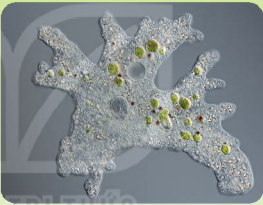
\includegraphics[width=4.3cm]{San_Pham/amoeba.png}
        };\\
        \vspace{0.15cm}
        {\fontsize{9.5}{12}\selectfont \textit{\color{gray!90!black}Trùng biến hình (\textit{Amoeba})}}
      \end{minipage}
      
      \vspace{0.25cm}
    \end{minipage}
  };
\end{tikzpicture}

&

% ===== COLUMN 2: CƠ THỂ ĐA BÀO =====
\begin{tikzpicture}
  \node[draw=borderBlue, fill=lightBlue!30, rounded corners=8pt, line width=1.2pt, inner sep=0pt] (card2) {
    \begin{minipage}{13.4cm}
      % Card Title
      \begin{tikzpicture}
        \node[fill=brandBlue, text=white, minimum width=13.4cm, minimum height=1.1cm, rounded corners=7pt] {
          {\fontsize{14}{17}\selectfont \textbf{CƠ THỂ ĐA BÀO (Ví dụ: Con voi, con gà, con người...)}}
        };
      \end{tikzpicture}
      
      \vspace{0.25cm}
      
      \begin{minipage}[t]{8.4cm}
        \fontsize{10.5}{15}\selectfont
        \begin{itemize}
          \setlength{\itemsep}{7pt}
          \setlength{\leftmargin}{0.3cm}
          \item[\color{brandBlue}$\blacktriangleright$] \textbf{\color{darkBlue}Kích thước cơ thể:} Thường có kích thước rất lớn.
          \item[\color{brandBlue}$\blacktriangleright$] \textbf{\color{darkBlue}Tỉ lệ $S/V$ (Diện tích / Thể tích):} \textbf{\color{red!70!black}RẤT NHỎ} (diện tích bề mặt rất nhỏ so với thể tích khổng lồ).
          \item[\color{brandBlue}$\blacktriangleright$] \textbf{\color{darkBlue}Cơ chế trao đổi chất:} Sự vận chuyển trực tiếp qua bề mặt ngoài \textbf{KHÔNG ĐỦ} cho các tế bào nằm sâu bên trong.
          \item[\color{brandBlue}$\blacktriangleright$] \textbf{\color{darkBlue}Tốc độ trao đổi chất:} Khuếch tán thụ động quá chậm, không cung cấp kịp dưỡng chất và oxi.
          \item[\color{brandBlue}$\blacktriangleright$] \textbf{\color{darkBlue}Mức độ chuyên hoá:} \textbf{BẮT BUỘC có các tế bào chuyên hoá} (hệ tuần hoàn, tiêu hoá, hô hấp...) để vận chuyển chất.
        \end{itemize}
      \end{minipage}%
      \hfill
      \begin{minipage}[t]{4.6cm}
        \centering
        \vspace{0.1cm}
        \tikz \node[draw=gray!30, rounded corners=6pt, inner sep=2pt, fill=white] {
          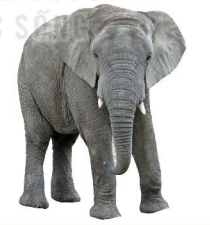
\includegraphics[width=4.0cm]{San_Pham/elephant.png}
        };\\
        \vspace{0.15cm}
        {\fontsize{9.5}{12}\selectfont \textit{\color{gray!90!black}Động vật đa bào (Con voi)}}
      \end{minipage}
      
      \vspace{0.25cm}
    \end{minipage}
  };
\end{tikzpicture}

\end{tabularx}

\vspace{0.4cm}

% ---------------- TAKEAWAY SUMMARY BOX ----------------
\begin{center}
\begin{tikzpicture}
  \node[draw=alertBorder, fill=alertBg, rounded corners=7pt, line width=1.2pt, inner sep=8pt] {
    \begin{minipage}{27.3cm}
      \fontsize{11}{15}\selectfont
      \textbf{\color{alertText}[!] BẢN CHẤT SINH HỌC CỐT LÕI:}\quad
      Khi kích thước cơ thể càng lớn $\longrightarrow$ Tỉ lệ diện tích bề mặt/thể tích ($S/V$) càng giảm $\longrightarrow$ Bề mặt tiếp xúc không đủ để trao đổi chất trực tiếp cho mọi tế bào $\longrightarrow$ Cơ thể đa bào bắt buộc phải hình thành \textbf{\color{red!70!black}CÁC TẾ BÀO VÀ CƠ QUAN CHUYÊN HOÁ} để tiếp nhận, vận chuyển và đào thải vật chất.
    \end{minipage}
  };
\end{tikzpicture}
\end{center}

\end{document}
